\section{Funktionalität}
SetlCup ist ein LR-Parser-Generator, welcher angelehnt an den bereits vorhandenen JavaCup ist.
Dabei ist die Idee wie folgt:
Der Benutzer von SetlCup erstellt durch eine gegebene Scanner- und Parserdefinition eine neue Setlx-Datei. Diese beinhaltet einen kanonischen LR-Parser, welcher auf den gegebenen Definitionen beruht. Anschließend kann eine Eingabedatei von dem generierten Parser überprüft werden. Dabei wird ggf. angegebener Code bei der Reduzierung der entsprechenden Regeln durchgeführt. 

Zunächst wird erklärt, wie die Komponente aufgerufen werden kann.
\section{Aufrufsmethoden}
Es gibt mehrere Möglichkeiten SetlCup aufzurufen:
\subsection{Aufruf über Kommandozeile}
\begin{enumerate}
	\item \begin{Verbatim}
	setlx setlcup.stlx -p parser_scanner_datei.stlx
	\end{Verbatim}
			Mit diesem Aufruf wird ein Parser gemäß der in der Eingabedatei gegebenen Definitionen erstellt.
	\item \begin{Verbatim}
	setlx setlcup.stlx -p parser_scanner_datei.stlx -d
	\end{Verbatim}
			Um die Art und Weise, wie der Parser generiert wird Nachzuvollziehen, kann mit der Option "`-d"' das Debugging eingeschaltet werden. Dabei wird empfohlen die Ausgabe in eine Datei umzuleiten.
	\item \begin{Verbatim}
	setlx parser_datei.stlx -p eingabe_datei.txt
	\end{Verbatim}
	Der erstellte Parser kann mit dem o.g. Befehl aufgerufen werden und probiert die Eingabedatei nach den angegebenen Regeln zu überprüfen.
		\item \begin{Verbatim}
	setlx parser_datei.stlx -p eingabe_datei.txt -d
	\end{Verbatim}
	Analog zur Parsererstellung wird durch die Option "`-d"' das Debugging eingeschaltet.
	\item \begin{Verbatim}
	setlx setlcup.stlx -h
	\end{Verbatim}
			Dieser Aufruf zeigt die Hilfe an, wie SetlCup aufgerufen werden kann.
	\item \begin{Verbatim}
	setlx test_setlcup.stlx
	\end{Verbatim}
			Dieser Aufruf testet die Funktionen des Parsergenerators mit den verschiedenen Beispielen.
\end{enumerate}
\section{Dateistruktur}
Der Parser-Generator SetlCup ist in mehrere Dateien aufgeteilt.
\paragraph{setlcup.stlx} Diese Datei wird aufgerufen, falls man über die Kommandozeile mit SetlCup arbeiten möchte. Sie nimmt die Parserdefinition als Parameter an und gibt sie an die jeweiligen Programme weiter, damit die Generierung des Parsers gestartet werden kann.
\paragraph{setlcup\_load.stlx} Diese Datei lässt zunächst den Scanner und daraufhin den Parser generieren. Falls über Setlx mit SetlCup gearbeitet werden soll, ist es möglich diese Datei als Grundlage zu nutzen. Sie wird u.a. für den Test der Funktionalität benutzt (siehe "test\_setlcup");
\paragraph{scanner\_generator.stlx} In dieser Datei wird die Eingabe analysiert. Es wird der Scanner aus den angegebenen Tokens generiert. Dieser wird daraufhin in einer Ausgabedatei abgelegt. Auch der Parser aus der Datei "\_sr\_parser\_part.stlx" wird der Datei angehangen. Zusätzlich wird die Grammatikdefinition analysiert und  in einer Token-Liste zurückgegeben.
\paragraph{parser\_generator.stlx} Der Parser Generator erstellt den kanonischen LR-Parser. Er erzeugt die notwendigen Action-, State- und Gototabellen. Diese werden zusammen mit den Regeln und dem vom User gewünschten Code auch in der o.g. Datei abgespeichert. 
\paragraph{\_sr\_parser\_part.stlx} Der Shift-Reduce-Parser ist in dieser Datei umgesetzt. Er wird zusammen mit den benötigten Tabellen, sowie dem Scanner in eine neue Datei kopiert. 
\paragraph{\_Grammar.stlx} In dieser Datei wird der erstelle Scanner und Parser abgelegt. Beim Aufruf wird die übergebene Datei geparsed. Dabei werden die o.g. Tabellen, sowie der vorher erstellte Scanner genutzt. Der Parser ist ein Shift-Reduce Parser. Beim Reducen wird der vom User angegebene Code ausgeführt. Der Wert der Variable "result" wird am Ende zurückgegeben.
\paragraph{test\_setlcup.stlx} Für einen Regressionstest kann mit dieser Datei überprüft werden ob alle Beispiele momentan geparsed werden können. Dabei wird zunächst für den arithmetischen Term der Parser erstellt. Dieser wird anschließend mit einer Eingabedatei aufgerufen und die Ergebnisse mit den vorher festgelegten verglichen. Das gleiche geschieht mit der Parserdefinition für eine einfache Programmiersprache.
\section{Aufbau der Definitionen}

Der Aufbau der Scanner- und Parserdefinitionen ist in drei Abschnitte zu unterteilen:
\begin{enumerate}
	\item Kommentare
	\item Scannerdefinition
	\item Parserdefinition
\end{enumerate}
\subsection{Kommentare}
Im obersten Bereich der Datei ist es möglich die Idee des Parsers zu beschreiben.
Dieser Abschnitt endet mit dem Symbol "`\%\%\%"'. 
\subsection{Scannerdefinition}
Der Scanner ist verantwortlich um zu Überprüfen, ob die Eingabedatei aus den angegebenen Tokens besteht. Die Syntax\mRefFigure{fig:scanner_def} wird im Folgenden erklärt.
\begin{figure}[!ht]
\begin{Verbatim}[ frame         = lines, 
                  framesep      = 0.3cm, 
                  labelposition = bottomline,
                  numbers       = left,
                  numbersep     = -0.2cm,
                  xleftmargin   = 0.8cm,
                  xrightmargin  = 0.8cm,
                ]
	INTEGER       := 0|[1-9][0-9]*     ;
	ASTERISK      := \*                ;
	WHITESPACE    := [ \t\v\r\s]       ;
	SKIP          := {WHITESPACE} | \n ;
\end{Verbatim}
\caption{Scanner Definition}
\label{fig:scanner_def}
\end{figure}
\begin{enumerate}
	\item In Zeile 1 wird der Token "INTEGER" definiert. Tokens werden auf die folgende Weise deklariert:\\
					token\_name := regex ; \\
					Dabei ist folgendes bei der Syntax des regulären Ausdrucks zu beachten:
					\begin{enumerate}
						\item Die Rückgabe der Capture-Gruppen z.B. "`ab\textbf{(.*)}ab"'	werden nicht unterstützt. Jedoch sind Nicht-Captures möglich: "`ab(\textbf{?:}.*)ab"'
						\item Die Nutzung der geschweiften Klammer wurde überlagert, sodass die regulären Ausdrücke der großgeschriebene Wörter innerhalb der Klammern im Nachhinein ersetz werden. Siehe Zeile 4 - "`\{TOKENNAME\}"'.
						\item Ansonsten sind die bereits in SetlX vorhandenen Regex-Ausdrücke benutzbar.
					\end{enumerate}
	\item Wie in SetlX (siehe Zeile 2 und 3) müssen auch in SetlCup vordefinierte Symbole wie "$*,+,?,|,\{,\},(,),\cdots$" escaped werden .
	\item In Zeile 4 wird "SKIP"-Token genutzt. In manchen Fällen werden gewisse Tokens nicht benötigt. Diese können mithilfe des "`SKIP"'-Tokens ignoriert werden. Dabei ist die Eingabe mit der o.g. Ersetzstrategie ( "` \{TOKENNAME\}"') oder die Nutzung eines regulären Ausdrucks möglich. Verschiedene Tokens müssen mit der Pipe "`|"' separiert werden.
\end{enumerate}

\subsection{Parserdefinition}
Die Definition der Grammatik für den Parser benutzt Konzepte aus JavaCup und ANTLR \mRefFigure{fig:example_grammer}.
\begin{figure}[!ht]
\begin{Verbatim}[ frame         = lines, 
                  framesep      = 0.3cm, 
                  labelposition = bottomline,
                  numbers       = left,
                  numbersep     = -0.2cm,
                  xleftmargin   = 0.8cm,
                  xrightmargin  = 0.8cm,
                ]
	grammar :=  definition_list;
  definition_list := rule_definition  definition_list
                    | ;
	rule_definition := RULEHEAD '::=' body_list ';' ;
	body_list := body '|' neBody_list
						| body
            | ;
  neBody_List := body body_list;
	body := element_list action_code;
  action_code := '{:' CODE ':}'
                | ;
  element_list := element element_list
              | ;
  element := token;
  token := LITERAL id
         | TOKEN_NAME id
         | RULE_HEAD id
         ;
  id := ':'ID_NAME
      |;
  RULE_HEAD := [a-z][a-zA-Z_0-9]*;
  TOKEN_NAME := [A-Z][A-Z_0-9]*;
  LITERAL := ''[^'']*'';
  ID_NAME := [a-z][a-zA-Z_0-9]*;
  CODE := [.\n]*;
\end{Verbatim}
\section{Beispiel parser}
\label{fig:example_grammer}
\end{figure}
\paragraph{RULE\_HEAD} beschreibt den Namen einer Regel z.B. "body". Somit können Regeln referenziert werden. 
\paragraph{TOKEN\_NAME} bezieht sich auf einen Token aus der Scanner Definition.
\paragraph{LITERAL}  beschreibt wortwörtliche Ausdrücke, welche genutzt werden können. 
\paragraph{ID\_NAME} ermöglicht es eine ID für den Rückgabewert einer Regel, bzw. eines Regex zu benutzen.
	% \begin{enumerate}
	% 	\item Token (defined in the scanner) e.g. "MINUS"
	% 	\item Token in  ' ' e.g. '+' as a literal
	% 	\item other rule\_heads e.g. "prod"
	% \end{enumerate}
	% The Tokens defined in the scanner, as well as the rule\_heads can have an id. This can be used in the action\_code.
\paragraph{action\_code} ist ein optionaler Teil einer Regel. Er kann am Ende einer Regel hinzugefügt werden. Der CODE innerhalb der Klammern  wird beim Reduzieren der Regel ausgeführt. Durch die Nutzung der Variable "`result"' können Ergebnisse zwischen den Regeln transferiert werden. Die IDs der Elemente der jeweiligen Regel können im Code benutzt werden. Der Code selber darf keine Anführungszeichen enthalten. Wenn sie doch notwendig sind, wird empfohlen sie zu escapen mit "$\backslash\backslash$" oder den Literalstring z.B. 'a+b = 15' zu nutzen. Außerdem sollte \textbf{generell} auf die Nutzung von Dollarzeichen verzichtet werden. Diese führen zu Komplikationen bei der Serialisierung des Parsers, da sie in SetlX eine Sonderfunktion einnehmen. 
	% \item[|] The pipe separates the different bodies.
\newpage
\subsection{Beispiele}
Das erste Beispiel beschreibt eine einfache arithmetische Grammatik.
Das zweite Beispiel beschreibt eine simple Programmiersprache.
\subsubsection{Arithmetische Ausdrücke}
Der arithmetische Parser \mRefFigure{fig:example_arithmetic_grammer} kann mit der oben beschriebenen Syntax definiert werden.
\begin{figure}[!ht]
\begin{Verbatim}[ frame         = lines, 
                  framesep      = 0.3cm, 
                  labelposition = bottomline,
                  numbers       = left,
                  numbersep     = -0.2cm,
                  xleftmargin   = 0.8cm,
                  xrightmargin  = 0.8cm,
                ]
  %%%

  INTEGER       := 0|[1-9][0-9]* ;
  WHITESPACE    := [ \t\v\r\s] ;


  SKIP          := {WHITESPACE} | \n ;

  %%%
  arith_expr 
   ::= expr_list:esl                {: result := ExprList(esl); :};

  expr_list 
   ::= expr_part:part expr_list:l {: result := [part] + l; :} 
     |                            {: result := []; :}
     ;
  expr_part 
   ::= expr:e ';'            {: result := e; :} ;
  expr 
   ::=  expr:e '+'  prod:p   {: result := Plus(e , p);  :} 
     |  expr:e '-'  prod:p   {: result := Minus(e , p); :} 
     |  prod:p               {: result := p;     :}
     ;
  prod 
   ::=  prod:p '*'  fact:f   {: result := Times(p , f); :}
     |  prod:p DIVIDE fact:f {: result := Div(p , f); :} 
     |  prod:p '%'    fact:f {: result := Mod(p , f); :} 
     |  fact:f               {: result := f;     :}
     ;
  fact 
   ::=  '(' expr:e_part ')'   {: result :=  e_part ;   :} 
     |  INTEGER:n             {: result := Integer(eval(n)); :} 
     ;
\end{Verbatim}
\caption{Parserdefinition für arithmetische Ausdrücke}
\label{fig:example_arithmetic_grammer}
\end{figure}
%\lstinputlisting[frame=single,numbers=left,basicstyle=\footnotesize]{math_expression_grammar_ast.g}
Eine beispielhafte Eingabe besteht aus drei verschiedenen mathematischen Termen \ref{fig:example_arithmetic_input}.
\begin{figure}[!ht]
\begin{Verbatim}[ frame         = lines, 
                  framesep      = 0.3cm, 
                  labelposition = bottomline,
                  numbers       = left,
                  numbersep     = -0.2cm,
                  xleftmargin   = 0.8cm,
                  xrightmargin  = 0.8cm,
                ]
  1 + 2 * 3 - 4;
  1 + 2 + 3 + 4;
  1 + ( 2 * 3 ) * 5 % 6;
\end{Verbatim}
\caption{Beispiel für arithmetische Terme}
\label{fig:example_arithmetic_input}
\end{figure}
Die Ausgabe des AST\mRefFigure{fig:arith_expr_tree} beschreibt die gezeigte Eingabe.
\begin{figure}[!ht]
	\centering
		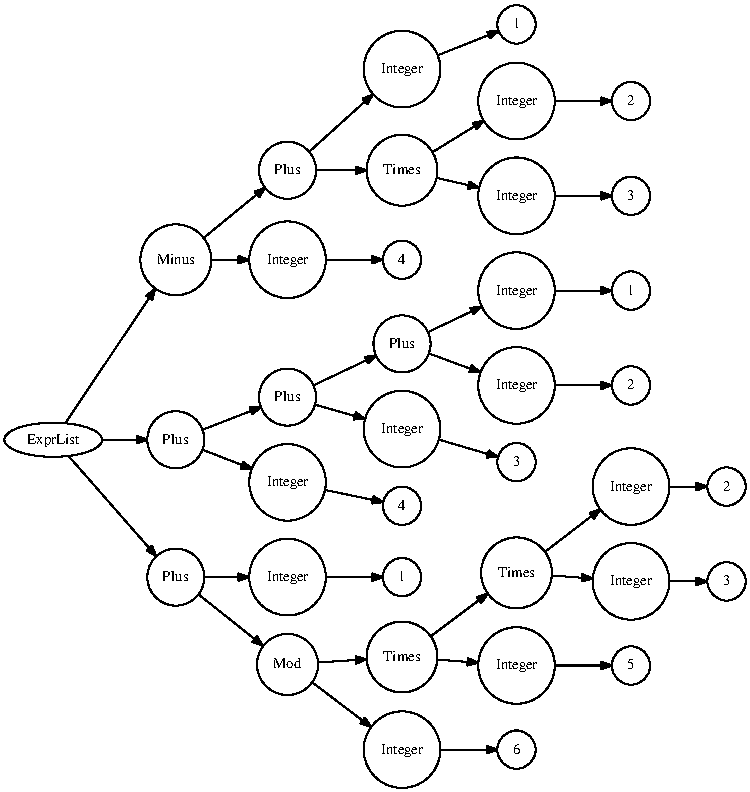
\includegraphics{arith_expr_tree.pdf}
	\caption{Arithexpr AST}
	\label{fig:arith_expr_tree}
\end{figure}

\subsubsection{Programmiersprachen Parser}
Der Scanner \mRefFigure{fig:example_interpreter_grammar_scanner} besteht aus den Tokens für Strings, Dezimalzahlen, Ganzzahlen usw.
Die Anwwisungen und Definitionen \mRefFigure{fig:example_interpreter_grammar_statements} beschreiben den Aufbau der Eingabedatei. Sie besteht aus Definitionen und Anweisungen.
Listen \mRefFigure{fig:example_interpreter_grammar_lists} sind zur Aneinanderreihung verschiedener Anweisungen, Definitionen, Ausdrücke etc. notwendig. 
Die Ausdrücke sind für boolsche, sowie arithmetische Terme notwendig \mRefFigure{fig:example_interpreter_grammar_expression}.
%\lstinputlisting[frame=single,numbers=left,basicstyle=\footnotesize ,breaklines=true]{interpreter_grammar_ast.g}
\begin{figure}[!ht]

\begin{Verbatim}[ frame         = lines, 
                  framesep      = 0.3cm, 
                  labelposition = bottomline,
                  numbers       = left,
                  numbersep     = -0.2cm,
                  xleftmargin   = 0.8cm,
                  xrightmargin  = 0.8cm,
                ]
  %%%
  STRING      := \"(?:\\.|[^\"])*\" ;
  WHITESPACE  := [ \t\v\r\s] ;
  INTEGER     := 0|[1-9][0-9]* ;
  DECIMAL     := 0\.[0-9]+|[1-9][0-9]*\.[0-9]+ ;
  ZID         := [a-zA-Z_][a-zA-Z0-9_]* ;

  SKIP        := {WHITESPACE}|\n|//[^\n]* ;
  %%%
\end{Verbatim}
\caption{Scannerdefinition für Programmiersprache}
\label{fig:example_interpreter_grammar_scanner}
\end{figure}
\begin{figure}[!ht]

\begin{Verbatim}[ frame         = lines, 
                  framesep      = 0.3cm, 
                  labelposition = bottomline,
                  numbers       = left,
                  numbersep     = -0.2cm,
                  xleftmargin   = 0.8cm,
                  xrightmargin  = 0.8cm,
                ]
  program 
    ::= dfnStmntList:d {: result := Program(d); :}
    ;

  dfnStmntList 
   ::= definition:d dfnStmntList:dl       {: result := [d] + dl; :}
     |  statement:stmts  dfnStmntList:dsl {: result := [stmts] + dsl; :}
     |                                    {: result := []; :}
     ;

  definition
   ::= 'function' ZID:function_name '(' paramList:param_list ')' 
      '{' stmntList:statement_list '}'
       {: result := Function(function_name, param_list, statement_list);:}
     ; 
  stmntList
    ::= statement:s stmntList:sl {: result := [s] + sl ; :}
     |  {: result := []; :}
     ;
  statement 
   ::= assignment:a ';'   {: result := Assign(a); :}    
     |  'print' '(' printExprList:printexpr_list ')' ';'      
                          {: result := Print(printexpr_list); :}
     |  'if' '(' boolExpr:b ')' '{' stmntList:st_list1 '}'    
                          {: result := If(b, st_list1); :}
     |  'while' '(' boolExpr:b ')' '{' stmntList:st_list2 '}' 
                          {: result := While(b, st_list2); :}
     |  'for' '(' assignment:i_a ';' boolExpr:b ';' assignment:e_a ')' 
		    '{' stmntList:st_list3 '}' 
                          {: result := For(i_a, b, e_a, st_list3);  :}
     |  'return' expr:e ';' {: result := Return(e); :}
     |  'return' ';'        {: result := Return();  :}
     |  expr:e ';'        {: result := Expr(e);   :}      
     |  'quit' ';'          {: result := Exit();    :}
     ;
\end{Verbatim}
\caption{Statements für Progammiersprachenparser}
\label{fig:example_interpreter_grammar_statements}
\end{figure}
\begin{figure}[!ht]

\begin{Verbatim}[ frame         = lines, 
                  framesep      = 0.3cm, 
                  labelposition = bottomline,
                  numbers       = left,
                  numbersep     = -0.2cm,
                  xleftmargin   = 0.8cm,
                  xrightmargin  = 0.8cm,
                ]
  printExprList 
   ::= printExpr:p ',' nePrintExprList:np {: result := [p] + np ; :}
     |  printExpr:p                       {: result := [p]; :}
     |                                    {: result := [];  :}
     ;
  nePrintExprList
   ::= printExpr:p                         {: result := [p]; :}
     |  printExpr:p ',' nePrintExprList:np {: result := [p] + np ; :}
     ;
  printExpr 
   ::= STRING:string {: result := PrintString(string); :}
     |  expr:e       {: result := e; :}
     ;
  assignment 
   ::= ZID:id '=' expr:e {: result := Assign(id, e); :}
     ;
  paramList 
   ::= ZID:id ',' neIDList:nid {: result := [id] + nid ; :}
     |  ZID:id                 {: result := [id] ; :}
     |                         {: result := []; :}
     ;
  neIDList
   ::= ZID:id ',' neIDList:nid {: result := [id] + nid ; :}
     |  ZID:id                 {: result := [id] ; :}
     ;
  exprList
   ::= expr:e ',' neExprList:el {: result := [e] + el; :}
     |  expr:e                  {: result := [e]; :}
     |                          {: result := [];  :}
     ;
  neExprList
   ::= expr:e ',' neExprList:el {: result := [e] + el; :}
     |  expr:e                  {: result := [e]; :}
     ;
		\end{Verbatim}
\caption{Listen für Progammiersprachenparser}
\label{fig:example_interpreter_grammar_lists}
\end{figure}
\begin{figure}[!ht]

\begin{Verbatim}[ frame         = lines, 
                  framesep      = 0.3cm, 
                  labelposition = bottomline,
                  numbers       = left,
                  numbersep     = -0.2cm,
                  xleftmargin   = 0.8cm,
                  xrightmargin  = 0.8cm,
                ]
  boolExpr 
   ::= expr:lhs '==' expr:rhs                {: result := Equation(lhs,rhs); :}
     |  expr:lhs '!=' expr:rhs               {: result := Inequation(lhs,rhs); :}
     |  disjunction:lhs '==' disjunction:rhs {: result := Equation(lhs,rhs); :}
     |  disjunction:lhs '!=' disjunction:rhs {: result := Inequation(lhs,rhs); :}
     |  expr:lhs '<=' expr:rhs               {: result := LessOrEqual(lhs,rhs);    :}
     |  expr:lhs '>=' expr:rhs               {: result := GreaterOrEqual(lhs,rhs); :}
     |  expr:lhs '<' expr:rhs                {: result := LessThan(lhs,rhs); :}
     |  expr:lhs '>' expr:rhs                {: result := GreaterThan(lhs,rhs); :}
     |  disjunction:d                        {: result := d; :}
     ;
  disjunction
   ::= disjunction:d '||' conjunction:c {: result := Disjunction(d,c); :}
     |  conjunction:c                   {: result := c; :}
     ;
  conjunction
   ::= conjunction:c '&&' boolFactor:f {:result := Conjunction(c,f); :}
     | boolFactor:f                    {: result := f; :}
     ;
  boolFactor
   ::= '(' boolExpr:be_par ')' {:  result := be_par; :}
     | '!' boolExpr:e          {: result := Negation(e); :}
     ;
  expr 
   ::= expr:e '+'   prod:p {: result := Sum(e,p); :} 
     |  expr:e '-'  prod:p {: result := Difference(e,p); :} 
     |  prod:p             {: result := p;     :}
     ;
  prod 
   ::= prod:p '*'  fact:f    {: result := Product(p,f); :}
     |  prod:p '\' fact:f    {: result := Quotient(p,f); :} 
     |  prod:p '%' fact:f    {: result := Mod(p,f); :} 
     |  fact:f               {: result := f;     :}
     ;
  fact 
   ::= '(' expr:e_par ')'            {: result := e_par;   :} 
     |  INTEGER:n                    {: result := Integer(eval(n));   :} 
     |  DECIMAL:d                    {: result := Decimal(eval(d)); :}
     |  ZID:id_1 '(' exprList:el ')' {: result := FunctionCall(id_1,el); :}
     |  ZID:id_2                     {: result := Variable(id_2); :}
     ;
		\end{Verbatim}
\caption{Ausdrücke für Progammiersprachenparser}
\label{fig:example_interpreter_grammar_expression}
\end{figure}
Ein Beispiel Programm \mRefFigure{fig:example_interpreter_input} zum Berechnen der Fakultät wird durch den Syntaxbaum \mRefFigure{fig:interpreter_tree} abgebildet.
\begin{figure}[!ht]

\begin{Verbatim}[ frame         = lines, 
                  framesep      = 0.3cm, 
                  labelposition = bottomline,
                  numbers       = left,
                  numbersep     = -0.2cm,
                  xleftmargin   = 0.8cm,
                  xrightmargin  = 0.8cm,
                ]
  function factorial(n) {
      if (n == 0) {
         return 1;
      }
      return n * factorial(n - 1);
  }
  print("Calculation of factorial for i = 1 to 9");
  for (i = 0; i < 10; i = i + 1) {
      print(i, "! = ", factorial(i));
  }
  print();
		\end{Verbatim}
\caption{Example interpreter input}
\label{fig:example_interpreter_input}
\end{figure}
%\lstinputlisting[frame=single,numbers=left,basicstyle=\footnotesize ,breaklines=true]{factorial.sl}
%The output AST  represents the syntactic structure of the factorial program. 
%\lstinputlisting[basicstyle=\footnotesize ,breaklines=true]{factorial_output.txt}


\begin{figure}[!ht]
	\centering
		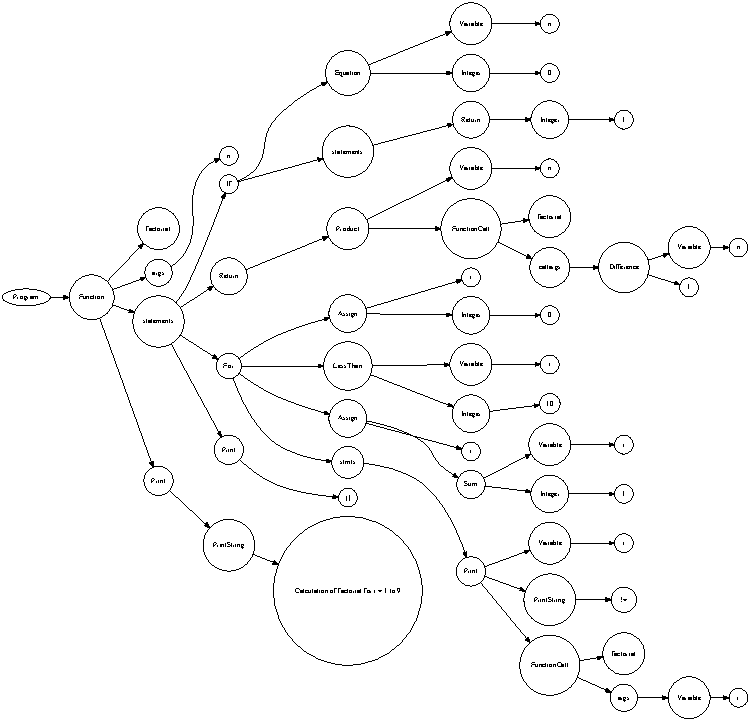
\includegraphics{interpreter_tree.pdf}
	\caption{Interpreter AST}
	\label{fig:interpreter_tree}
\end{figure}

